\documentclass{article}

% Language setting
% Replace `english' with e.g. `spanish' to change the document language
\usepackage[french]{babel}

% Set page size and margins
% Replace `letterpaper' with `a4paper' for UK/EU standard size
\usepackage[letterpaper,top=2cm,bottom=2cm,left=3cm,right=3cm,marginparwidth=1.75cm]{geometry}

% Useful packages
\usepackage{amsmath}
\usepackage{graphicx}
\usepackage[colorlinks=true, allcolors=blue]{hyperref}

\title{Your Paper}
\author{You}

\begin{document}

\begin{center}
    \huge IA pour jeu de stratégie : approche algorithmique contre
    apprentissage machine.
\end{center}

\vspace{1cm}

\begin{center}
  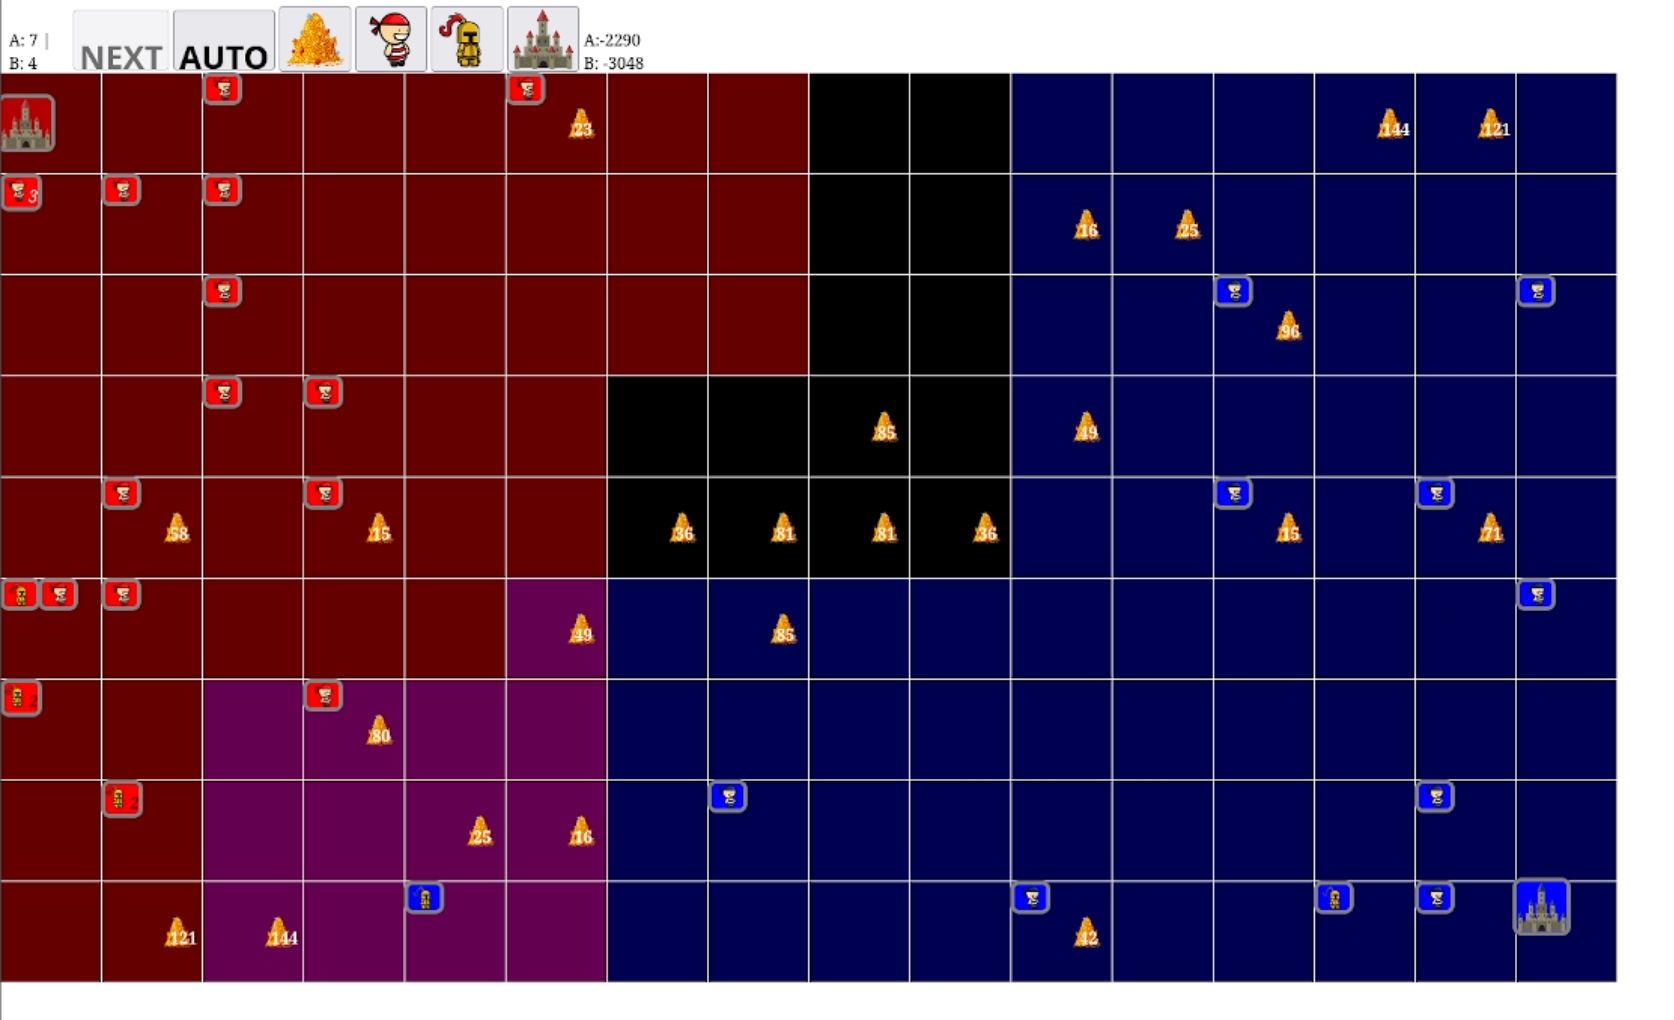
\includegraphics[width=0.9\linewidth]{match}
  
  Capture d'écran d'une partie de ChartiChaud
\end{center}

\noindent \textbf{Encadrant·es :} Louis JACHIET (INFRES) et Nils HOLZENBERGER (INFRES)\\
\noindent \textbf{Nombre d'étudiant·es minimum dans chaque instance de
  ce projet :} 2\\
\noindent \textbf{Nombre d'étudiant·es maximum dans chaque instance de ce projet :} 4\\
\noindent \textbf{Combien d'instances de ce projet :} 2\\
\noindent \textbf{Mots clefs :} IA, Machine-Learning, Jeu, TBS, Algorithmique, Programmation


\section{Contexte}

\paragraph{Un peu d'histoire.}
Les jeux de stratégie sont des jeux avec des règles et un objectif
précis qui définissent un petit univers parfaitement maîtrisable, facile à reproduire sur ordinateur. Pour ces raisons, les jeux
offrent une manière très pratique de mesurer les progrès en
intelligence artificielle et de comparer diverses approches. Leur
popularité permet aussi une médiatisation et ainsi les avancées en IA
arrivent souvent aux oreilles du grand public à la suite de
compétitions : Deep Blue d'IBM aux échecs au milieu des années 90,
Watson d'IBM en 2011 à Jeopardy!, AlphaGo de Deepmind en 2012 au
Go. Plus récemment, on peut aussi citer AlphaStar de Deepmind sur le
jeu vidéo Starcraft II ou Five d'Open AI sur Dota 2, même si ces
dernières n'ont pas vraiment dépassé les meilleurs joueurs et
joueuses.

Dans le domaine de l'IA pour les jeux, on peut distinguer deux grandes
approches :
\begin{itemize}
\item une qui est plutôt \emph{algorithmique} où un·e expert·e va définir
  une stratégie globale que l'ordinateur appliquera (par exemple à
  l'aide de divers algorithmes pour énumérer de nombreuses
  possibilités ou de systèmes de planifications) ;
\item une qui ressort plutôt de \emph{l'apprentissage machine} où l'on va
  construire un système d'IA qui va apprendre petit à petit en jouant
  contre d'autres IA, contre elle-même ou en regardant un nombre
  important de parties.
\end{itemize}
Cette classification binaire est évidemment imparfaite, chaque IA
pouvant emprunter aux deux, mais jusqu'au début des années 2010,
l'approche algorithmique était largement privilégiée tandis que, suite
aux augmentations des capacités de calcul et l'amélioration des
algorithmes, les méthodes à base d'apprentissage machine se sont petit
à petit imposées.

\paragraph{Objectif du projet.}
% Suffisamment bien entraînées et bien développées, les méthodes à base d'apprentissage sont fréquemment meilleures sur le type du jeu que l'on va étudier mais elles sont souvent aussi assez difficiles à mettre en œuvre.
L'objectif de ce projet est d'avoir deux groupes qui
travaillent sur deux IA pour le même jeu. Un des deux groupes
utilisera une approche plutôt algorithmique tandis que l'autre
s'attaquera au problème avec l'approche apprentissage machine. Les
deux IA s'affronteront régulièrement pour voir quelle IA est meilleure
au jeu. Il sera aussi possible de jouer directement (contre l'IA ou
non) pour s'entraîner, l'entraîner et mieux comprendre le jeu.

\paragraph{Jeu étudié.}

Le jeu étudié est en cours de développement. Une version jouable se
trouve à l'adresse suivante :
\url{https://gitlab.telecom-paris.fr/louis.jachiet/chartichaud}
et un premier match peut être vu ici :
\url{https://peertube.r2.enst.fr/w/gpG2zBA1k1N7yP6pB58YMZ}.

\section{Livrables du projet}

\paragraph{Premier livrable : une IA.}
Le principal objectif du projet est de voir ce que des élèves de
Télécom en première année sont capables de faire comme IA, avec
chacune des deux approches. Les groupes devront donc développer une IA
pour le jeu considéré. Cette IA sera à développer de façon continue
pendant toute la période du projet (et pas seulement à la toute fin !)
car des matchs seront régulièrement organisés, mesurant leurs niveaux
relatifs.

\paragraph{Deuxième livrable : un (petit) rapport.}

Un objectif secondaire est de s'inspirer de l'existant et donc de
faire une rapide revue de l'état de l'art pour la construction d'IA
pour les jeux de stratégie. Bien que le jeu étudié dans ce projet ait
été créé spécifiquement pour le projet et donc qu'il n'existe
actuellement aucune IA dont on puisse s'inspirer, de nombreuses IA ont
été faites pour divers types de jeux et il est possible de s'en
inspirer. En parallèle du code de l'IA, chaque groupe devra écrire un
petit rapport contenant une synthèse en quelques pages des méthodes
proposées dans l'état de l'art pour les jeux de stratégie et leur
applicabilité au jeu considéré.

Comme le projet va sûrement mener à diverses pistes considérées,
implémentées puis parfois abandonnées, nous demandons à ce que le
rapport soit complété d'une analyse des différentes pistes et
algorithmes qui ont été utilisés à un moment ou à un autre en
détaillant les temps de développement et d'entraînement qui ont été
nécessaires pour chacune des pistes.

\paragraph{Remarques finales.}
L'objectif du projet est d'avoir une comparaison entre les deux
approches, il n'est donc pas possible que les deux équipes travaillent
sur la même approche. Les personnes affectées à ce projet risquent
de ne pas avoir le choix de l'approche.

La performance des algorithmes des deux équipes sera mesurée
régulièrement par des matchs tout au long du projet. L'équipe
encadrante souhaite qu'il y ait une émulation pour avoir la meilleure
IA à ce jeu, mais la notation ne s'appuiera pas sur la comparaison
entre les performances des deux IA.

\end{document}
